%%%%%%%%%%%%%%%%%%%%%%%%%%%%%%%%%%%%%%%%%
% Journal Article
% 
% Gahan M. Saraiya
% 18MCEC10
%
% References
% ==========
% 
%%%%%%%%%%%%%%%%%%%%%%%%%%%%%%%%%%%%%%%%%
\documentclass[a4paper,11pt,oneside]{Thesis}
%\usepackage[a4paper]{geometry}
\usepackage[utf8]{inputenc}
\usepackage[english]{babel}
%\usepackage{lipsum}
%\usepackage{listings}

\usepackage{graphicx}
\graphicspath{ {./assets/} {./pics/} {./eps/} {./figures/}}
%\usepackage{epsfig}
%\usepackage{epstopdf}



%%%%%%%%%%%%%%%%%%%%%%%%%%%%%%%%%%%%%%%%%%%%%%%%%%
%% COLOR DEFINITIONS
%%%%%%%%%%%%%%%%%%%%%%%%%%%%%%%%%%%%%%%%%%%%%%%%%%
\usepackage[svgnames]{xcolor} % Enabling mixing colors and color's call by 'svgnames'
%%%%%%%%%%%%%%%%%%%%%%%%%%%%%%%%%%%%%%%%%%%%%%%%%%
\definecolor{MyColor1}{rgb}{0.2,0.4,0.6} %mix personal color
\newcommand{\textb}{\color{Black} \usefont{OT1}{lmss}{m}{n}}
\newcommand{\blue}{\color{MyColor1} \usefont{OT1}{lmss}{m}{n}}
\newcommand{\blueb}{\color{MyColor1} \usefont{OT1}{lmss}{b}{n}}
\newcommand{\red}{\color{LightCoral} \usefont{OT1}{lmss}{m}{n}}
\newcommand{\green}{\color{Turquoise} \usefont{OT1}{lmss}{m}{n}}
%%%%%%%%%%%%%%%%%%%%%%%%%%%%%%%%%%%%%%%%%%%%%%%%%%




%%%%%%%%%%%%%%%%%%%%%%%%%%%%%%%%%%%%%%%%%%%%%%%%%%
%% FONTS AND COLORS
%%%%%%%%%%%%%%%%%%%%%%%%%%%%%%%%%%%%%%%%%%%%%%%%%%
%    SECTIONS
%%%%%%%%%%%%%%%%%%%%%%%%%%%%%%%%%%%%%%%%%%%%%%%%%%
%\usepackage{titlesec}
%\usepackage{sectsty}
%%%%%%%%%%%%%%%%%%%%%%%%
%%set section/subsections HEADINGS font and color
%\sectionfont{\color{MyColor1}}  % sets colour of sections
%\subsectionfont{\color{MyColor1}}  % sets colour of sections
%
%%set section enumerator to arabic number (see footnotes markings alternatives)
%\renewcommand\thesection{\arabic{section}.} %define sections numbering
%\renewcommand\thesubsection{\thesection\arabic{subsection}} %subsec.num.
%
%%define new section style
%\newcommand{\mysection}{
%    \titleformat{\section} [runin] {\usefont{OT1}{lmss}{b}{n}\color{MyColor1}} 
%    {\thesection} {3pt} {} } 

% Glossaries build
\usepackage[acronym]{glossaries}
\makeglossaries
\loadglsentries{sections/glossaries}


\usepackage{longtable}
\renewcommand\thesection{\Roman{section}} % Roman numerals for the sections
\renewcommand\thesubsection{\Roman{subsection}} % Roman numerals for subsections
%----------------------------------------------------------------------------------------
%       DATE FORMAT
%----------------------------------------------------------------------------------------
\usepackage{datetime}
\newdateformat{monthyeardate}{\monthname[\THEMONTH], \THEYEAR}
%----------------------------------------------------------------------------------------

%\titleformat{\section}[block]{\large\scshape\centering}{\thesection.}{1em}{} % Change the look of the section titles
%\titleformat{\subsection}[block]{\large}{\thesubsection.}{1em}{} % Change the look of the section titles
%\newcommand{\horrule}[1]{\rule{\linewidth}{#1}} % Create horizontal rule command with 1 argument of height
%\usepackage{fancyhdr} % Headers and footers
%\pagestyle{fancy} % All pages have headers and footers
%\fancyhead{} % Blank out the default header
%\fancyfoot{} % Blank out the default footer



%%%%%%%%%%%%%%%%%%%%%%%%%%%%%%%%%%%%%%%%%%%%%%%%%%
%		CAPTIONS
%%%%%%%%%%%%%%%%%%%%%%%%%%%%%%%%%%%%%%%%%%%%%%%%%%
%\usepackage{caption}
%%\usepackage{subcaption}
%%%%%%%%%%%%%%%%%%%%%%%%%
%\captionsetup[figure]{labelfont={color=Turquoise}}

%%%%%%%%%%%%%%%%%%%%%%%%%%%%%%%%%%%%%%%%%%%%%%%%%%
%		!!!EQUATION (ARRAY) --> USING ALIGN INSTEAD
%%%%%%%%%%%%%%%%%%%%%%%%%%%%%%%%%%%%%%%%%%%%%%%%%%
%using amsmath package to redefine eq. numeration (1.1, 1.2, ...) 
%%%%%%%%%%%%%%%%%%%%%%%%

%\renewcommand{\theequation}{\thesection\arabic{equation}}
%
%%set box background to grey in align environment 
%\usepackage{etoolbox}% http://ctan.org/pkg/etoolbox
%\makeatletter
%\patchcmd{\@Aboxed}{\boxed{#1#2}}{\colorbox{black!15}{$#1#2$}}{}{}%
%\patchcmd{\@boxed}{\boxed{#1#2}}{\colorbox{black!15}{$#1#2$}}{}{}%
%\makeatother

%%%%%%%%%%%%%%%%%%%%%%%%%%%%%%%%%%%%%%%%%%%%%%%%%%

% -------------------------------------------------------------------------------
% *** FLOWCHART AND GRAPHS PACKAGES ***
% -------------------------------------------------------------------------------
\usepackage{tikz}
\usepackage{pgfplots}
\usepackage{neuralnetwork}
\pgfplotsset{compat=1.5.1}
\usetikzlibrary{snakes, arrows, shapes, shapes.geometric, calc, automata, positioning}
\tikzstyle{startstop} = [rectangle, rounded corners, minimum height=1cm, minimum width=2cm, 
text centered, trapezium stretches=true, draw=black, 
%fill=red!30
]

\tikzstyle{io} = [trapezium, trapezium left angle=70, trapezium right angle=110, minimum width=3cm, trapezium stretches=true, minimum height=1cm, text centered, draw=black, 
%fill=blue!30
]
\tikzstyle{process} = [rectangle, minimum width=3cm, minimum height=1cm, text centered, draw=black, trapezium stretches=true, 
%fill=orange!30
]
\tikzstyle{decision} = [diamond, minimum width=3cm, minimum height=1cm, text centered, draw=black, trapezium stretches=true, 
%fill=green!30
]
\tikzstyle{arrow} = [thick,->,>=stealth]
\pgfplotsset{every axis/.append style={tick label style={/pgf/number format/fixed},font=\scriptsize,ylabel near ticks,xlabel near ticks,grid=major}}
\tikzset{%
	every neuron/.style={
		circle,
		draw,
		minimum size=1cm
	},
	neuron missing/.style={
		draw=none, 
		scale=4,
		text height=0.333cm,
		execute at begin node=\color{black}$\vdots$
	},
}
% -------------------------------------------------------------------------------

% -------------------------------------------------------------------------------
% *** INDIAN RUPEE SYMBOL ***
% -------------------------------------------------------------------------------
\usepackage{tfrupee} 
% ------------ INDIAN RUPEE SYMBOL END ---------------------------


% -------------------------------------------------------------------------------
% SET UP MATH Commands and configs
% -------------------------------------------------------------------------------


\usepackage{amsmath, amssymb, amsfonts, amsthm, fouriernc, mathtools}
% mathtools for: Aboxed (put box on last equation in align envirenment)
%\usepackage{microtype} %improves the spacing between words and letters

\usepackage{theorem}
% Special Matrix
\newenvironment{spmatrix}[1]
{\def\mysubscript{#1}\mathop\bgroup\begin{bmatrix}}
	{\end{bmatrix}\egroup_{\textstyle\mathstrut\mysubscript}}
% Adding explaination below equation terms
\newcommand{\explain}[2]{\underbrace{#1}_{\parbox{\widthof{$#1$}}{\tiny#2}}}
%\newcommand{\explain}[2]{\underbrace{#1}_{\parbox{\widthof{#1}}{\footnotesize\raggedright #2}}}

%%%%%%%%%%%%%%%%%%%%%%%%%%%%%%%%%%%%%%%%%%%%%%%%%%
%% DESIGN CIRCUITS
%%%%%%%%%%%%%%%%%%%%%%%%%%%%%%%%%%%%%%%%%%%%%%%%%%
%\usepackage[siunitx, american, smartlabels, cute inductors, europeanvoltages]{circuitikz}
%%%%%%%%%%%%%%%%%%%%%%%%%%%%%%%%%%%%%%%%%%%%%%%%%%



%\makeatletter
%\let\reftagform@=\tagform@
%\def\tagform@#1{\maketag@@@{(\ignorespaces\textcolor{red}{#1}\unskip\@@italiccorr)}}
%\renewcommand{\eqref}[1]{\textup{\reftagform@{\ref{#1}}}}
%\makeatother
%\usepackage{hyperref}
%\hypersetup{colorlinks=true}

% to allow adding line break in table cell

\usepackage{makecell}
%\hypersetup{%
%  colorlinks=true,
%  linkcolor=blue,
%  linkbordercolor={0 0 1}
%}
% 
\renewcommand\lstlistingname{Algorithm}
\renewcommand\lstlistlistingname{Algorithms}
\def\lstlistingautorefname{Alg.}

\lstdefinestyle{Python}{
    language        = Python,
    frame           = lines, 
    basicstyle      = \footnotesize,
    keywordstyle    = \color{blue},
    stringstyle     = \color{green},
    commentstyle    = \color{red}\ttfamily
}

%\setlength{\parindent}{0.0in}
%\setlength{\parskip}{0.05in}

%%%%%%%%%%%%%%%%%%%%%%%%%%%%%%%%%%%%%%%%%%%%%%%%%%
%% PREPARE TITLE
%%%%%%%%%%%%%%%%%%%%%%%%%%%%%%%%%%%%%%%%%%%%%%%%%%
\title{
%	\blue Project Report \\
    \blueb Generic IP independent BIOS Signing and Parsing}
\author{Gahan Saraiya (18MCEC10)}
\date{\monthyeardate\today}
%\date{March, 2019}

%%%%%%%%%%%%%%%%%%%%%%%%%%%%%%%%%%%%%%%%%%%%%%%%%%
%----------------------------------------------------------------------------------------
%       SET HEADER AND FOOTER
%----------------------------------------------------------------------------------------
\newcommand\theauthor{Gahan Saraiya}
\newcommand\thesubject{Generic IP independent BIOS Signing and Parsing}
\renewcommand{\footrulewidth}{0.4pt}% default is 0pt
\fancyhead[C]{Institute of Technology, Nirma University $\bullet$ \monthyeardate\today} % Custom header text
\fancyfoot[LE,LO]{\thesubject}
\fancyfoot[RO,LE]{Page \thepage} % Custom footer text
%----------------------------------------------------------------------------------------

\renewcommand\theadalign{bc}
\renewcommand\theadfont{\bfseries}
\renewcommand\theadgape{\Gape[4pt]}
\renewcommand\cellgape{\Gape[4pt]}
\newcommand*\tick{\item[\Checkmark]}
\newcommand*\arrow{\item[$\Rightarrow$]}
\newcommand*\fail{\item[\XSolidBrush]}
\usepackage{minted} % for highlighting code sytax
\definecolor{LightGray}{gray}{0.9}
%\renewcommand*{\arraystretch}{2}
%\definecolor{LightGray}{gray}{0.9}

\setminted[text]{
	frame=lines, 
	breaklines,
	baselinestretch=1.2,
	bgcolor=LightGray,
%	fontsize=\small
}
\setminted[bash]{
%	frame=lines, 
	breaklines,
	baselinestretch=1.2,
	bgcolor=LightGray,
%	fontsize=\small
}
\setminted[python]{
	frame=lines, 
	breaklines, 
	linenos,
	baselinestretch=1.2,
%	bgcolor=LightGray,
%	fontsize=\small
}


\usepackage[square, numbers, comma, sort&compress]{natbib}  
\usepackage{verbatim}  % Needed for the "comment" environment to make LaTeX comments
% Allows "\bvec{}" and "\buvec{}" for "blackboard" style bold vectors in maths
\hypersetup{urlcolor=blue, colorlinks=true}  % Colours hyperlinks in blue, but this can be distracting if there are many links.

\begin{document}
	\maketitle
	
	
	\setstretch{1.0}
	\fancyhead{}
	\rhead{\thepage}
	\lhead{}
	
	\pagestyle{fancy}
	
	
\Declaration{

\addtocontents{toc}{\vspace{1em}}  

\vspace{1cm}

I hereby declare that the dissertation {\bf \textit{\thesubject}} submitted by me to the \theinstitute, \theuniversity, Ahmedabad, 382481 in partial fulfillment of the requirements for the award of {\bf \thedegree} in {\bf \thebranch with specialization in \thebranch} is a bona-fide record of the work carried out by me under the supervision of {\bf\textit{Prof. Dvijesh Bhatt}}. \\
I further declare that the work reported in this dissertation, has not been submitted and will not be submitted, either in part or in full, for the award of any other degree or diploma of this institute or of any other institute or University.

\vspace{1cm}

Sign:\\
%\rule[1em]{25em}{0.5pt}  % This prints a line for the signature

Name \& Roll. No.:\\
%\rule[1em]{25em}{0.5pt}  % This prints a line for the signature
 
Date: \\
%\rule[1em]{25em}{0.5pt}  % This prints a line to write the date
\thispagestyle{empty} 
}

\clearpage  % Abstract ended, start a new page

	
	\Certificate{
\addtocontents{toc}{\vspace{0.5em}}  % Add a gap in the Contents, for aesthetics

This is to certify that the dissertation entitled {\bf \textit{\thesubject}} 
submitted by {\bf \textit{\theauthor}  
(Roll No. \therollno)} 
to \theuniversity Ahmedabad, in partial fulfullment of the requirement for the award of
the degree of {\bf Master of Technology} in
{\bf Computer Science \& Engineering with specialization in Computer Science \& Engineering}  
is a bona-fide work carried out under my supervision.
The dissertation fulfills the requirements as per the regulations of this
University and in my opinion meets the necessary standards for submission.
The contents of this dissertation have not been submitted and will not be submitted
either in part or in full, for the award of any other degree or diploma
and the same is certified.

\vspace{2cm}
%
%   Spaces for signatures 
%
\begin{tabular}{ l p{2.1cm} l p{3cm} l }
	Prof. Dvijesh Bhatt & \hspace{0.3cm} & Dr. Priyanka Sharma & & 
	\\ Guide \& Assistant Professor, & &  Professor, & & 
	\\ CSE Department, & & Coordinator M.Tech - CSE (CSE) & &
	\\ \theinstitute, & & \theinstitute, & &
	\\ \theuniversity, Ahmedabad. & & \theuniversity, Ahmedabad & &
	\\
\end{tabular}
}

\vspace{2cm}
%
%   Spaces for signatures 
%

\begin{tabular}{ l p{3.1cm}lp{4cm}l }
	Dr. Madhuri Bhavsar & \hspace{0.3cm} & Dr. Alka Mahajan & &
	\\ Professor and Head, & & Director, & &
	\\ CSE Department, & & \theinstitute, & &
	\\ \theinstitute, & & \theuniversity, Ahmedabad & &
	\\ \theuniversity, Ahmedabad. & & & &
\end{tabular}
\thispagestyle{empty}
\clearpage  

	
	
\addtotoc{Abstract} 
\abstract{
\addtocontents{toc}{\vspace{1em}}  

Intel System on a Chip (\gls{soc}) features a new set of Intel Intellectual Property (\gls{ip}) for every generation. \gls{bios} involves development of major individual components such as Processor, Graphics/Memory Controller, Input/Output Controller hub, System Monitor/Management Bus, Direct Media Interface, SATA/IDE/USB, Peripheral Component Interconnect (\gls{pci}), Voltage Regulator and Advanced Configuration and Power Interface (\gls{acpi}) for every Intel System on a Chip (\gls{soc}). Section \ref{section-introduction} describes all the basic information required on the Intel \gls{soc}.

Section \ref{section-design} involves the design of the Basic Boot Flow of the BIOS followed by Section \ref{section-architecture} and Section \ref{section-smm} explains the architecture and protocols which are the concept used to build the proposed framework which is described under Section \ref{section-proposed-work} to aid the development and debugging iteration for various stakeholders including but not limited to BIOS Developers, Validation Engineers, Automation team. 

The framework is designed and implemented to aid the development process by eliminating longer duration of common debugging steps and providing a sophisticated way to build and test the various scenarios includes but not limited to Setup Options, Firmware Flashing, UEFI Variable Creation.

}

\clearpage  
	
	
\acknowledgements{
\addtocontents{toc}{\vspace{1em}} 

It gives me immense pleasure in expressing thanks and profound gratitude to Prof. Dvijesh Bhatt, Assistant Professor, Computer Engineering Department, \theinstitute,  \theuniversity,  Ahmedabad for his valuable guidance and continual encouragement throughout this work. The appreciation and continual support he has imparted has been a great motivation to me in reaching a higher goal.  His guidance has triggered and nourished my intellectual maturity that I will benefit from, for a long time to come. 

It gives me an immense pleasure to thank Dr. Madhuri Bhavsar, Honorable Head of Computer Science And Engineering Department, \theinstitute, \theuniversity, Ahmedabad for her kind support and providing basic infrastructure and healthy research environment.

A special thank you is expressed whole heartedly to Dr.  Alka Mahajan,  Honorable Director, \theinstitute, \theuniversity, Ahmedabad for the unmentionable motivation she has extended throughout course of this work. I would  also thank the Institution, all faculty members of Computer Engineering Department, \theuniversity, Ahmedabad for their special attention and suggestions towards the project work.

\vspace{2cm}

\begin{flushright}
    \theauthor

    \therollno
\end{flushright}
}

\clearpage  % End of the Acknowledgements
%% ----------------------------------------------------------------

	\pagestyle{fancy}  
	
	\lhead{\emph{Contents}}  
	\tableofcontents  % Write out the Table of Contents

	\section{Introduction}
\subsection{Uncore Intellectual Properties}
Intel System on a Chip (SoC) features a new set of Intel Uncore Intellectual Property (IP)
for every generation. The Uncore encompasses system agent (SA), memory and Uncore agents
such as graphics controller, display controller, memory controller and Input Output (IO). The
Uncore IPs are Peripheral Component Interface Express (PCIe), Graphics Processing Engine
(GPE), Thunderbolt, Imaging Processing Agent (IPU), North Peak (NPK), Virtualization
Technology for directed-IO (Vt-d), Volume Management Device (VMD).

PCI Express abbreviated as PCIe or PCI-E, is designed to replace the older PCI standards.
A data communication system is developed for use the transfer data between the host and the
peripheral devices via PCIe. Thunderbolt is the brand name of a hardware interface developed
by Intel that allows the connection of external peripherals to a computer. Thunderbolt combines
PCI Express (PCIe) and DisplayPort (DP) into two serial signals, and additionally provides DC
power, all in one cable. Graphics Processing Engine (GPE), Integrated graphics, shared graphics
solutions, integrated graphics processors (IGP) or unified memory architecture (UMA) utilize a
portion of a computer's system RAM rather than dedicated graphics memory. GPEs can be
integrated onto the motherboard as part of the chipset. Virtual Technology for Directed-IO (Vt-d)
is an input/output memory management unit (IOMMU) allows guest virtual machines to directly
use peripheral devices, such as Ethernet, accelerated graphics cards, and hard-drive controllers,
through DMA and interrupt remapping.

\subsection{Legacy \gls{bios} and \gls{uefi}}

\paragraph{\gls{bios}} is the dominant standard which defines a firmware interface.

"Legacy" (as in Legacy \gls{bios}), in the context of firmware specifications, refer to an older, widely used specification. Major responsibility of \gls{bios} is to set up the hardware, load and start an \gls{os}. When the system boots, the BIOS initializes and identifies system devices including video display card, mouse, hard disk drive, keyboard, solid state drive and other hardware followed by locating software held on a boot device i.e. a hard disk or removable storage such as CD/DVD or USB and loads and executes that software, giving it control of the computer. This process is also referred to as "booting" or "boot strapping".

\subsubsection{Background of Legacy \gls{bios}}
In 1980s, IBM developed the personal computer with a 16-bit BIOS with the aim of ending the BIOS after the first 250,000 products. Legacy BIOS is based upon Intel's original 16-bit architecture, ordinarily referred to as  "8086" architecture. And as technology advanced, Intel extended that 8086 architecture from 16 to 32-bit.
Legacy BIOS is able to run different \gls{os}, such as MS-DOS, equally well on systems other than IBM. Additionally, Legacy BIOS has a defined OS-independent interface for hardware that enables interrupts to communicate with video, disk and keyboard services along with the BIOS ROM loader and bootstrap loader, to name a few.

Use of legacy BIOS is diminishing and is expected to be phased out in new systems by the year 2020.

\subsubsection{Limitations of legacy BIOS}
Over the years, many new configuration and power management technologies were integrated
into BIOS implementations as well as support for many generations of Intel® architecture
hardware. However certain limitations of BIOS implementations such as 16-bit addressing mode,
1 MB addressable space, PC AT hardware dependencies and upper memory block (UMB)
dependencies persisted throughout the years. The industry also began to have need for methods to
ensure quality of individual firmware modules as well as the ability to quickly integrate libraries
of third-party firmware modules into a single platform solution across multiple product lines.
These inherent limitations and existing market demands opened the opportunity for a fresh BIOS
architecture to be developed and introduced to the market. The UEFI specifications and resulting
implementations have begun to effectively address these persisting market needs.

One of the critical maintenance challenges for BIOS is that each implementation has tended to
be highly customized for the specific motherboard on which it is deployed. Moving component
modules across designs typically requires significant porting, integration, testing and debug work.
This is one of the markets challenges the UEFI architecture promises to address.

\subsection{Unified Extensible Firmware Interface (\gls{uefi})}
\gls{uefi} was developed as a replacement for legacy BIOS to streamline the booting process, and act as the interface between a operating system and its platform firmware. It not only replaces most BIOS functions, but also offers a rich extensible pre-OS environment with advanced boot and runtime services.
Unified Extensible Firmware Interface (\gls{uefi}) is grounded in Intel's initial Extensible Firmware Interface (EFI) specification 1.10, which defines a software interface between an operating system and platform firmware. The UEFI architecture allows users to execute applications on a command line interface. It has intrinsic networking capabilities and is designed to work with multi-processors (MP) systems.

\begin{figure}[h]
	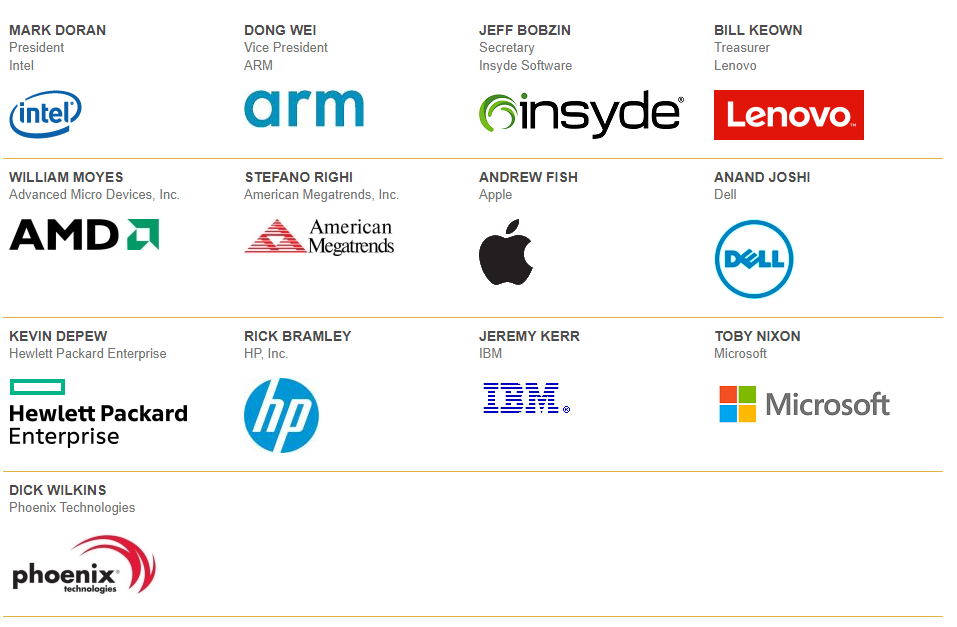
\includegraphics[width=\linewidth]{uefi_board_of_directors}
	\caption{Board of Directors of UEFI Forum}\label{fig:introduction-uefi-board-of-directors}
\end{figure}

The UEFI Forum board of directors consists of representatives from 11 industry leaders as described in Figure \ref{fig:introduction-uefi-board-of-directors}. These involved organizations work to ensure that the UEFI specifications meet industry needs.

UEFI uses a different interface for boot services and runtime services but UEFI does not specify how "Power On Self Test" (POST) and Setup are implemented - those are BIOS' primary functions.

\subsubsection{\gls{uefi} Driver Model Extension}
Access to boot devices is provided through a set of protocol interfaces. One purpose of the
UEFI Driver Model is to provide a replacement for \verb|PC-AT|-style option ROMs. It is important
to point out that drivers written to the UEFI Driver Model are designed to access boot devices in
the pre-boot environment. They are not designed to replace the high-performance, OS-specific
drivers.

The UEFI Driver Model is designed to support the execution of modular pieces of code,
also known as drivers, that run in the pre-boot environment. These drivers may manage or control
hardware buses and devices on the platform, or they may provide some software-derived, platform specific service. The UEFI Driver Model also contains information required by UEFI driver writers to design and implement any combination of bus drivers and device drivers that a platform
might need to boot a UEFI-compliant OS.

The UEFI Driver Model is designed to be generic and can be adapted to any type of bus or
device. The UEFI Specification describes how to write PCI bus drivers, PCI device drivers, USB
bus drivers, USB device drivers, and SCSI drivers. Additional details are provided that allow UEFI
drivers to be stored in PCI option ROMs, while maintaining compatibility with legacy option ROM
images.

One of the design goals in the UEFI Specification is keeping the driver images as small as
possible. However, if a driver is required to support multiple processor architectures, a driver
object file would also be required to be shipped for each supported processor architecture. To
address this space issue, this specification also defines the EFI Byte Code Virtual Machine. A
UEFI driver can be compiled into a single EFI Byte Code object file. UEFI Specificationcomplaint firmware must contain an EFI Byte Code interpreter. This allows a single EFI Byte
Code object file that supports multiple processor architectures to be shipped. Another space saving
technique is the use of compression. This specification defines compression and decompression
algorithms that may be used to reduce the size of UEFI Drivers, and thus reduce the overhead
when UEFI Drivers are stored in ROM devices.

The information contained in the UEFI Specification can be used by OSVs, IHVs, OEMs,
and firmware vendors to design and implement firmware conforming to this specification, drivers
that produce standard protocol interfaces, and operating system loaders that can be used to boot
UEFI compliant operating systems.

\subsubsection{\gls{uefi}'s Role in boot process}

During the boot process, UEFI speaks to the operating system loader and acts as the interface between the operating system and the BIOS.

The \verb|PC-AT| boot environment presents significant challenges to innovation within the
industry. Each new platform capability or hardware innovation requires firmware developers to
craft increasingly complex solutions, and often requires OS developers to make changes to their
boot code before customers can benefit from the innovation. This can be a time-consuming process
requiring a significant investment of resources. The primary goal of the UEFI specification is to
define an alternative boot environment that can alleviate some of these considerations. In this goal, the specification is like other existing boot specifications.

\subsection{Comparing of Legacy \gls{bios} and \gls{uefi}}

\begin{table}
	\centering
	\renewcommand{\arraystretch}{2}
	\caption{Legacy BIOS v/s UEFI}\label{table:legacy-bios-vs-uefi}
	\begin{tabular}{l | p{5cm} | p{5cm}}
		& Legacy BIOS & EFI
		\\ \hline \hline
		Language & Assembly & C ($ 99\% $)
		\\ \hline
		Resource & Interrupt Hardcode Memory Access hardcore I/O Access & Diver, Protocols
		\\ \hline
		Processor & x86 16-bit & CPU Protects Mode (Flat Mode)
		\\ \hline
		Expand & Hook Interrupt & Load Driver
		\\ \hline
		OS Bridge & ACPI & Run Time Driver Software
		\\ \hline
		$ 3^{rd} $ Party ISV \& IHV & Bas for Support & Easy for Support and for Multi Platforms
		\\ \hline
	\end{tabular}
\end{table}


\subsection{Advanced Configuration and Power Interface (\gls{acpi})}
The ACPI Component Architecture (ACPICA) defines and implements a group of software
components that together create an implementation of the ACPI specification. A major goal of the
architecture is to isolate all operating system dependencies to a relatively small translation or
conversion layer (the OS Services Layer) so that the bulk of the ACPICA code is independent of
any individual operating system. Therefore, hosting the ACPICA code on new operating systems
requires no source changes within the ACPICA code itself.

The components of the architecture include:
\begin{itemize}
	\item An OS-independent, kernel-resident ACPICA Subsystem component that provides the fundamental ACPI services such as the AML interpreter and namespace management.
	\item An OS-dependent OS Services Layer for each host operating system to provide OS support for the OS-independent ACPICA Subsystem.
	\item An ASL compiler-disassembler for translating ASL code to AML byte code and for disassembling existing binary ACPI tables back to ASL source code.
	\item Several ACPI utilities for executing the interpreter in ring 3 user space, extracting binary ACPI tables from the output of the ACPI Dump utility, and translating the ACPICA source	code to Linux/Unix format.
\end{itemize}

In Figure \ref{fig:introduction-acpi-component-architecture}, the ACPICA subsystem is shown in relation to the host operating system, device driver, OSPM software, and the ACPI hardware

\begin{figure}[h]
	\centering
	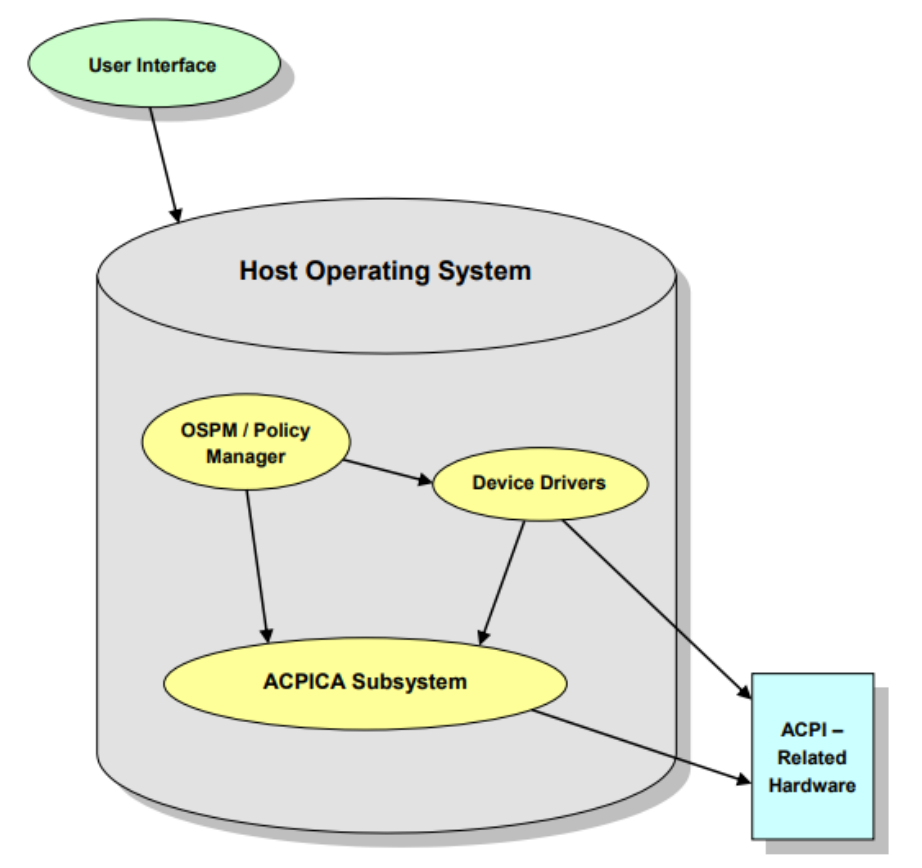
\includegraphics[width=0.7\linewidth]{introduction/acpi-component-architecture}
	\caption{The \gls{acpi} Component Architecture}\label{fig:introduction-acpi-component-architecture}
\end{figure}

\subsubsection{Overview of ACPICA Subsystem}
The ACPICA Subsystem implements the low level or fundamental aspects of the ACPI
specification. Included are an AML parser/interpreter, ACPI namespace management, ACPI table
and device support, and event handling. Since the ACPICA subsystem provides low-level system
services, it also requires low-level operating system services such as memory management,
synchronization, scheduling, and I/O.

To allow the ACPICA Subsystem to easily interface to any operating system that provides such
services, an Operating System Services Layer translates ACPICA-to-OS requests into the system
calls provided by the host operating system. The OS Services Layer is the only component of the
ACPICA that contains code that is specific to a host operating system.

Thus, the ACPICA Subsystem consists of two major software components:
\begin{itemize}
	\item The basic kernel-resident ACPICA Subsystem provides the fundamental ACPI services	that are independent of any particular operating system.
	\item The OS Services Layer (OSL) provides the conversion layer that interfaces the OS independent ACPICA Subsystem to a host operating system.
\end{itemize}

When combined into a single static or loadable software module such as a device driver or
kernel subsystem, these two major components form the ACPICA Subsystem. Throughout this
document, the term "ACPICA Subsystem" refers to the combination of the OS-independent
ACPICA Subsystem with an OS Services Layer components combined into a single module,
driver, or load unit.

\subsubsection{OS-independent ACPICA Subsystem}
The OS-independent ACPICA Subsystem supplies the major building blocks or subcomponents that are required for all ACPI implementations — including an AML interpreter, a namespace manager, ACPI event and resource management, and ACPI hardware support.

One of the goals of the ACPICA Subsystem is to provide an abstraction level high enough such
that the host operating system does not need to understand or know about the very low-level ACPI
details. For example, all AML code is hidden from the host. Also, the details of the ACPI hardware
are abstracted to higher-level software interfaces.

The ACPICA Subsystem implementation makes no assumptions about the host operating system or environment. The only way it can request operating system services is via interfaces provided by the OS Services Layer.

The primary user of the services provided by the ACPICA Subsystem are the host OS device drivers and power/thermal management software.

\subsubsection{Operating System Services Layer}
The OS Services Layer (or OSL) operates as a translation service for requests from the OS independent ACPICA subsystem back to the host OS. The OSL implements a generic set of OS service interfaces by using the primitives available from the host OS. Because of its nature.

The OS Services Layer must be implemented anew for each supported host operating
system. There is a single OS-independent ACPICA Subsystem, but there must be an OS Services
Layer for each operating system supported by the ACPI component architecture.

The primary function of the OSL in the ACPI Component Architecture is to be the small
glue layer that binds the much larger ACPICA Subsystem to the host operating system. Because
of the nature of ACPI itself — such as the requirement for an AML interpreter and management
of a large namespace data structure — most of the implementation of the ACPI specification is
independent of any operating system services. Therefore, the OS-independent ACPICA Subsystem
is the larger of the two components.

The overall ACPI Component Architecture in relation to the host operating system is Figure

\begin{figure}[h]
	\centering
	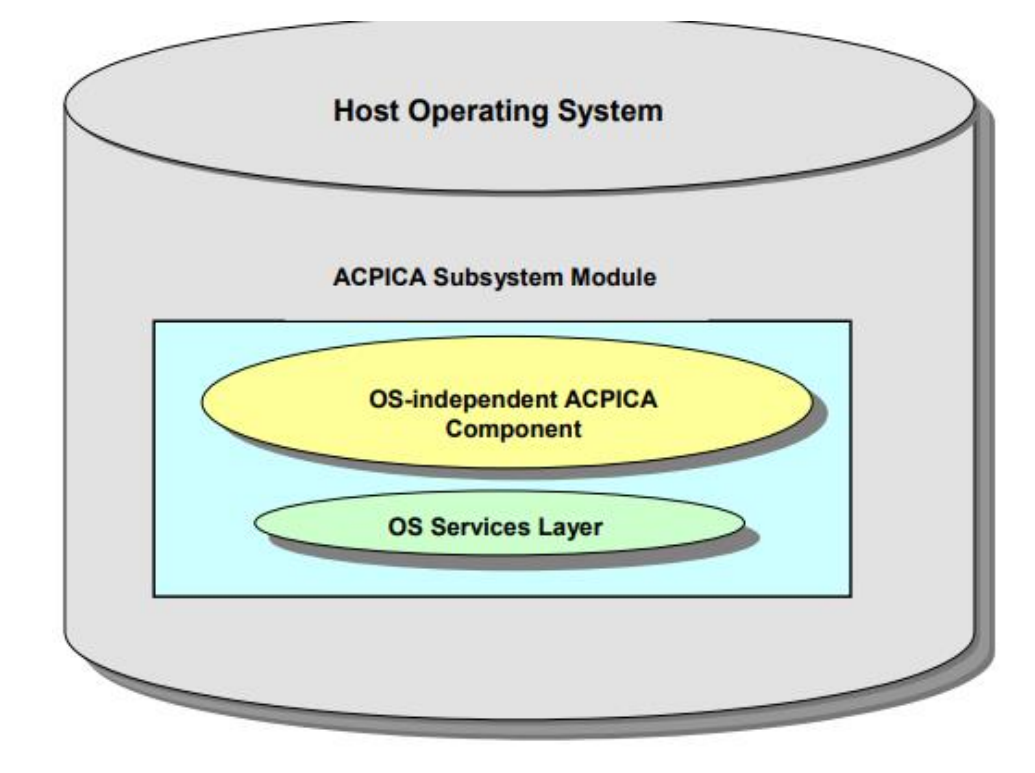
\includegraphics[width=0.7\linewidth]{introduction/acpica-subsystem-architecture}
	\caption{ACPICA Subsystem Architecture}\label{fig:introduction-acpica-subsystem-architecture}
\end{figure}

\subsubsection{ACPICA Subsystem Interaction}
The ACPICA Subsystem implements a set of external interfaces that can be directly called from
the host OS. These Acpi* interfaces provide the actual ACPI services for the host. When operating
system services are required during the servicing of an ACPI request, the Subsystem makes
requests to the host OS indirectly via the fixed AcpiOs* interfaces. The diagram below illustrates
the relationships and interaction between the various architectural elements by showing the flow
of control between them. Note that the OS-independent ACPICA Subsystem never calls the host directly instead it makes calls to the AcpiOs * interfaces in the OSL. This provides the ACPICA
code with OS-independence.

The Interaction between the Architectural Components Is shown in Figure \ref{fig:-introduction-acpi-interaction-between-the-architectural-components}

\begin{figure}[h]
	\centering
	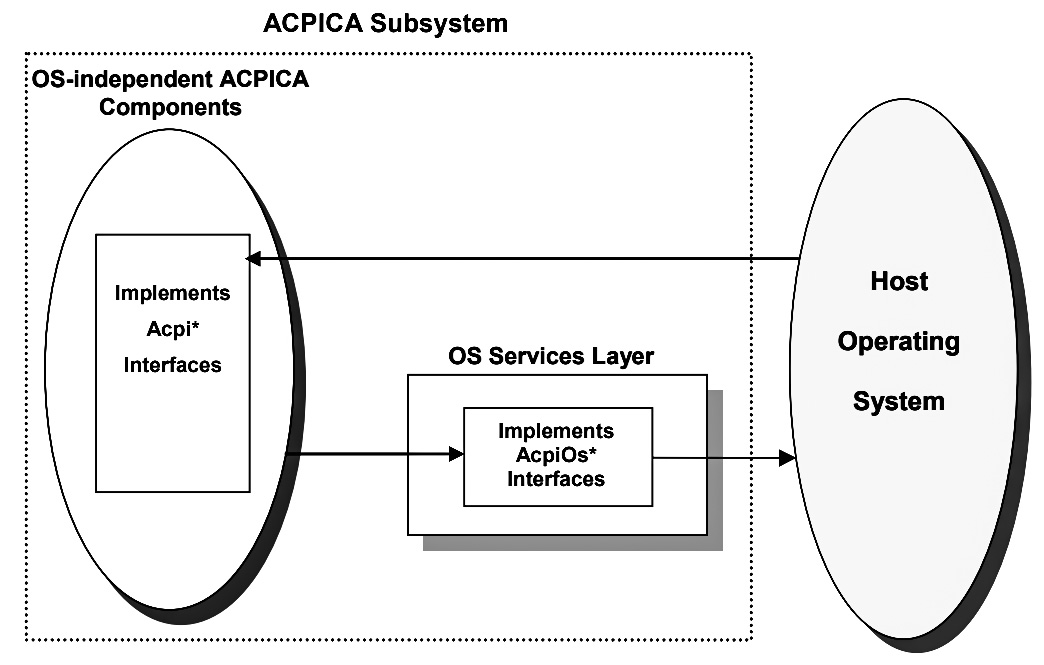
\includegraphics[width=0.7\linewidth]{introduction/acpi-interaction-between-the-architectural-components}
	\caption{Interaction between the Architectural Components}\label{fig:-introduction-acpi-interaction-between-the-architectural-components}
\end{figure}




	\section{Design}

\subsection{\gls{uefi}/\gls{pi} Firmware Images}
\gls{uefi} and \gls{pi} specifications define the standardized format for EFI firmware storage devices (FLASH or other non-volatile storage) which are abstracted into "Firmware Volumes". Build systems must be capable of processing files to create the file formats described by the \gls{uefi} and PI specifications. The tools provided as part of the \gls{edk2} BaseTools package process files compiled by third party tools, as well as text and Unicode files in order to create UEFI or PI compliant binary image files. In some instances, where UEFI or PI specifications do not have an applicable input file format, such as the Visual Forms Representation (VFR) files used to create PI compliant IFR content, tools and documentation have been provided that allows the user to write text files that are processed into formats specified by UEFI or PI specifications.

\begin{figure}[h]
	\centering
	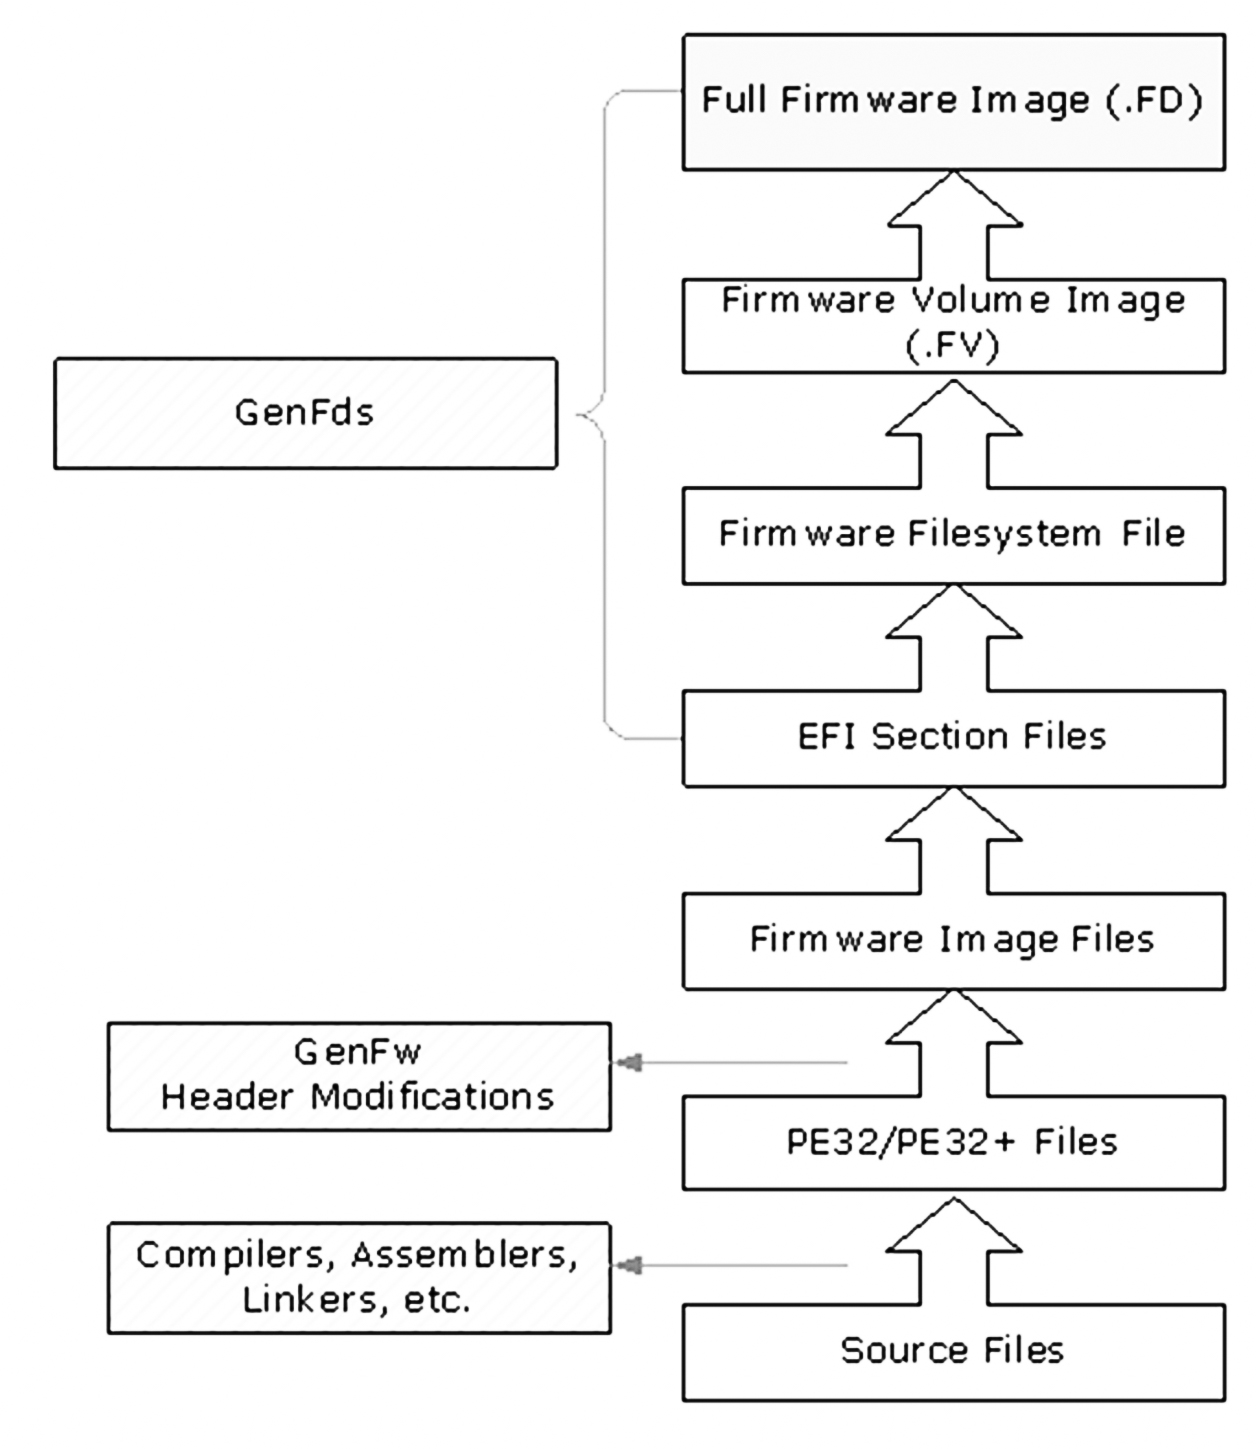
\includegraphics[width=0.7\linewidth]{design/uefi-pi-firmware-image-creation}
	\caption{UEFI/PI Firmware Image Creation}\label{fig:design-uefi-pi-firmware-image-creation}
\end{figure}

A Firmware Volume (FV) is a file level interface to firmware storage. Multiple FVs may be present in a single FLASH device, or a single FV may span multiple FLASH devices. An FV may be produced to support some other type of storage entirely, such as a disk partition or network device. For more information consult the Platform Initialization Specification, Volume 3.
In all cases, an FV is formatted with a binary file system. The file system used is typically the Firmware File System (FFS), but other file systems may be possible in some cases. Hence, all modules are stored as "files" in the FV. Some modules may be "execute in place" (linked at a fixed address and executed from the ROM), while others are relocated when they are loaded into memory and some modules may be able to run from ROM if memory is not present (at the time of the module load) or run from memory if it is available.
Files themselves have an internally defined binary format. This format allows for implementation of security, compression, signing, etc. Within this format, there are one or more "leaf" images. A leaf image could be, for example, a PE32 image for a DXE driver.

Therefore, there are several layers of organization to a full UEFI/PI firmware image. These layers are illustrated below in Figure \ref{fig:design-uefi-pi-firmware-image-creation}. Each transition between layers implies a processing step that transforms or combines previously processed files into the next higher level. Also shown in Figure \ref{fig:design-uefi-pi-firmware-image-creation} are the reference implementation tools that process the files to move them between the different layers.

\begin{figure}[h]
	\centering
	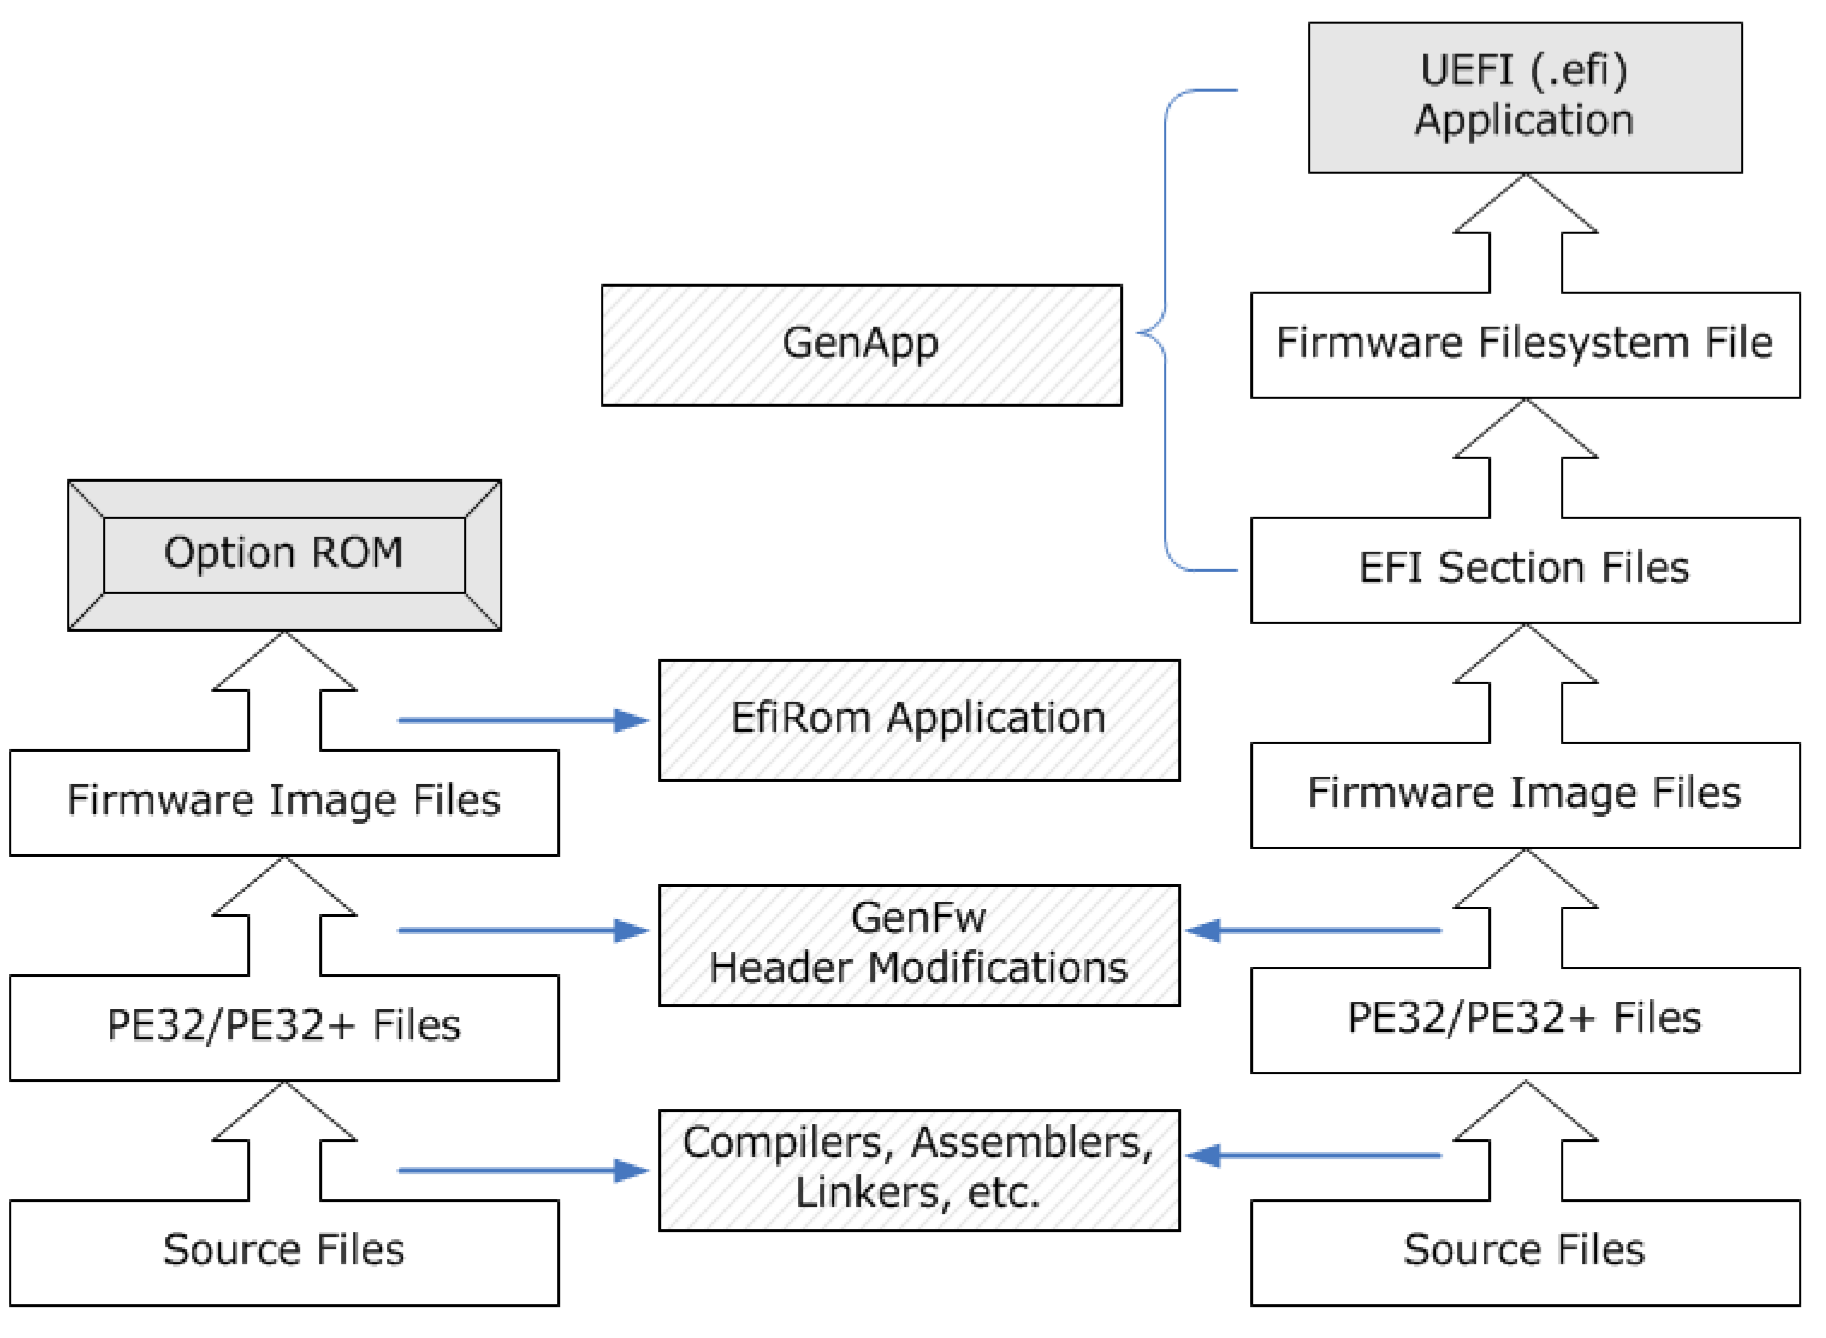
\includegraphics[width=0.7\linewidth]{design/efi-application-creation}
	\caption{UEFI/PI Firmware Image Creation}\label{fig:design-efi-application-creation}
\end{figure}


In addition to creating images that initialize a complete platform, the build process also supports creation of stand-alone UEFI applications (including OS Loaders) and Option ROM images containing driver code. Figure \ref{fig:design-efi-application-creation}, below, shows the reference implementation tools and creation processes for both of these image types

The final feature that is supported by the EDK II build process is the creation of Binary Modules that can be packaged and distributed for use by other organizations. Binary modules do not require distribution of the source code. This will permit vendors to distribute UEFI images without having to release proprietary source code.

This packaging process permits creation of an archive file containing one or more binary files that are either Firmware Image files or higher (EFI Section files, Firmware File system files, etc.). The build process will permit inserting these binary files into the appropriate level in the build stages.

\subsection{Platform Initialization \gls{pi} Boot Sequence}
PI compliant system firmware must support the six phases: security (\gls{sec}), pre-efi initialization (\gls{pei}), driver execution environment (\gls{dxe}), boot device selection (\gls{bds}), run time (RT) services and After Life (transition from the OS back to the firmware) of system. Refer to Figure \ref{fig:design-pi-boot-phases} below.

\begin{figure}[h]
	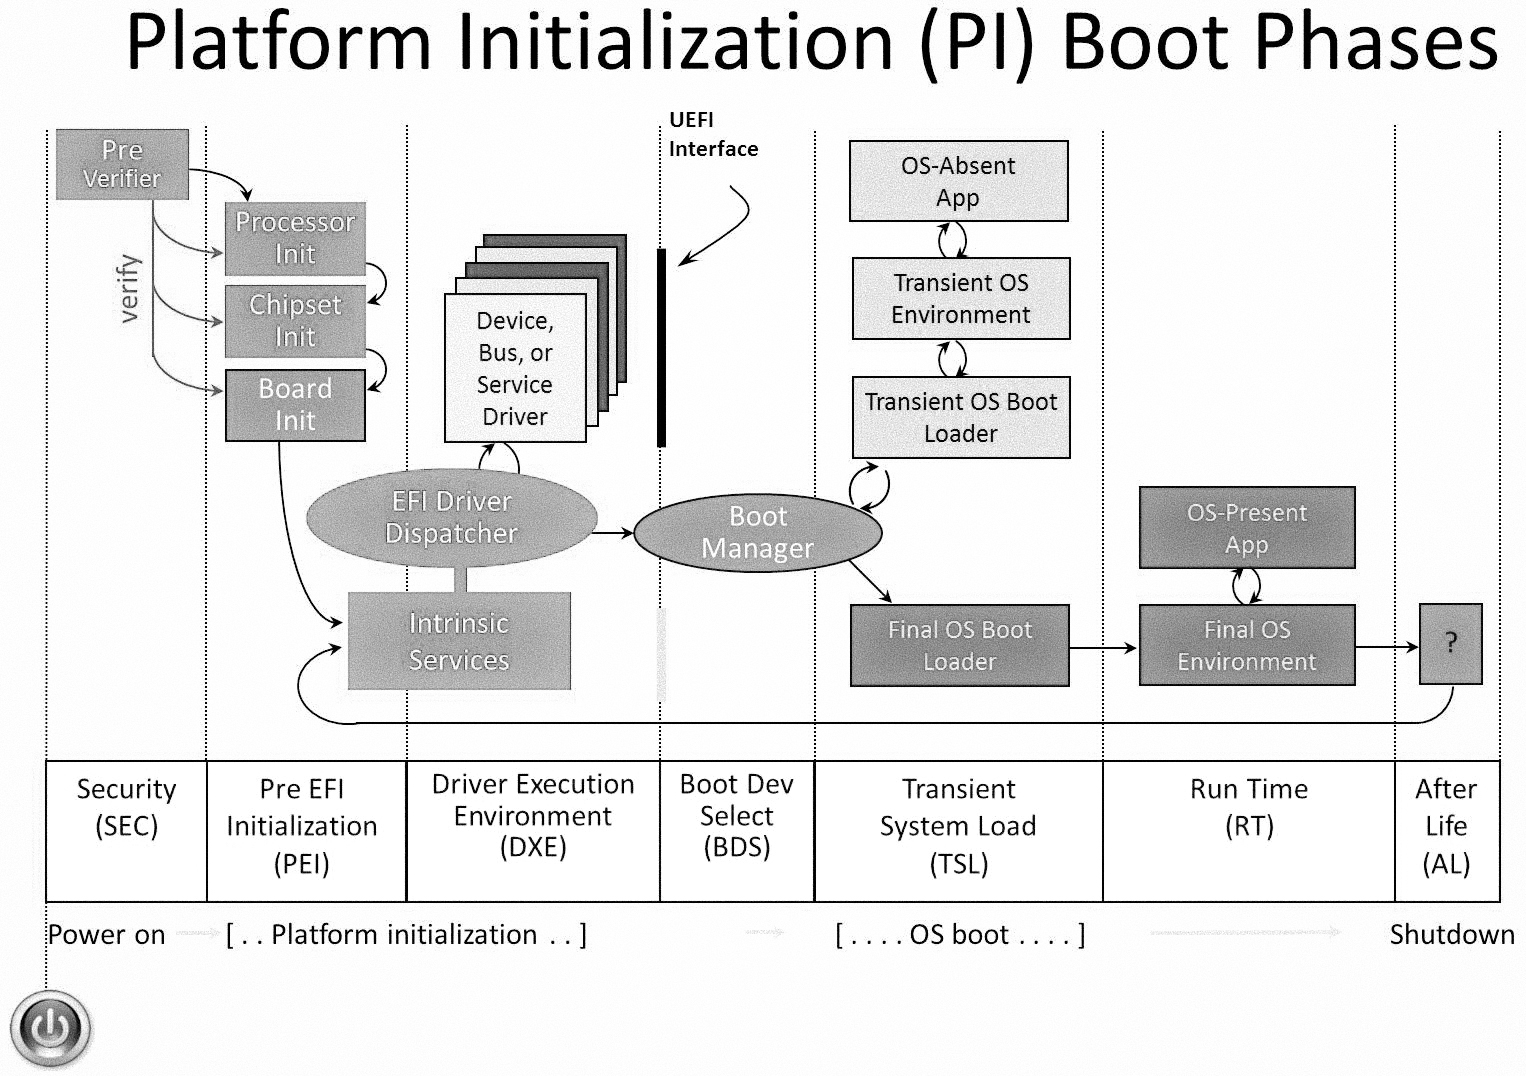
\includegraphics[width=\linewidth]{PI_Boot_Phases}
	\caption{\gls{pi} Boot Phases}\label{fig:design-pi-boot-phases}
\end{figure}

\subsection{Security (\gls{sec})}
The Security (SEC) phase is the first phase in the PI Architecture and is responsible for the following:
\begin{itemize}
	\item Handling all platform restart events
	\item Creating a temporary memory store
	\item Serving as the root of trust in the system
	\item Passing handoff information to the PEI Foundation
\end{itemize}
The security section may contain modules with code written in assembly. Therefore, some EDK II module development environment (MDE) modules may contain assembly code. Where this occurs, both Windows and GCC versions of assembly code are provided in different files

\subsection{Pre-EFI Initialization (\gls{pei})}
The Pre-EFI Initialization (PEI) phase described in the PI Architecture specifications is invoked quite betimes in the boot period. Specifically, after about preliminary processing in the Security (SEC) phase, any machine restart event will invoke the PEI phase.
The PEI phase is designed to be developed in many parts and consists of:
\begin{itemize}
	\item PEI Foundation (core code)
	\item Pre-EFI Initialization Modules (specialized plug-ins)
\end{itemize}
The PEI phase initially operates with the platform in a nascent state, leveraging only on-processor resources, such as the processor cache as a call stack, to dispatch Pre-EFI Initialization Modules (PEIMs).

The PEI phase cannot assume the availability of amounts of memory (RAM) as DXE and hence PEI phase limits its support to the following:
\begin{itemize}
	\item Locating and validating PEIMs
	\item Dispatching PEIMs
	\item Facilitating communication between PEIMs
	\item Providing handoff data to later phases
\end{itemize}

These PEIMs are responsible for the following:
\begin{itemize}
	\item Initializing some permanent memory complement
	\item Describing the memory in Hand-Off Blocks (HOBs)
	\item Describing the firmware volume locations in HOBs
	\item Passing control into the Driver Execution Environment (DXE) phase
\end{itemize}

Figure \ref{fig:design-pei-operation-diagram} shows a diagram describes the action carried out during the PEI phase

\begin{figure}[h]
	\centering
	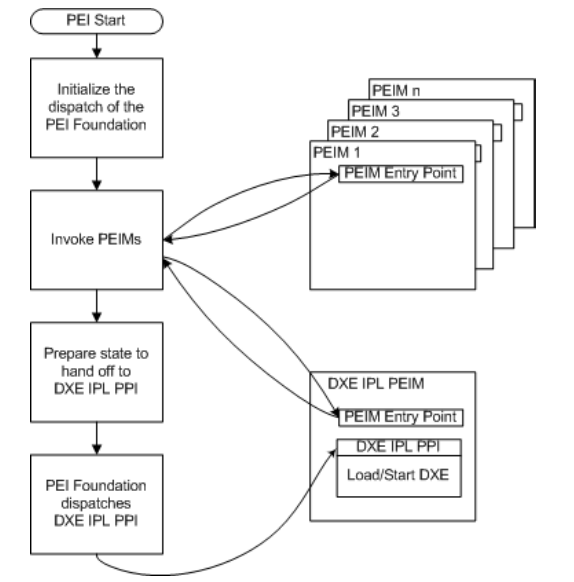
\includegraphics[width=0.7\linewidth]{design/pei-operation-diagram}
	\caption{Diagram of PI Operations}\label{fig:design-pei-operation-diagram}
\end{figure}

\subsubsection{PEI Services}
The PEI Foundation establishes a system table named the PEI Services Table that is visible to all Pre-EFI Initialization Modules (PEIMs) in the system. A PEI Service is defined as a function, command, or other capability manifested by the PEI Foundation when that service’s initialization requirements are met. Because the PEI phase has no permanent memory available until nearly the end of the phase, the range of services created during the PEI phase cannot be as rich as those created during later phases. Because the location of the PEI Foundation and its temporary RAM is not known at build time, a pointer to the PEI Services Table is passed into each PEIM’s entry point and also to part of each PEIM-to-PEIM Interface (PPI). 

The PEI Foundation provides the classes of services listed in Table \ref{table:design-pei-foundation-class-service}

\begin{table}[h]
	\centering
	\begin{tabular}{ l | p{8cm} }
		Service & Details
		\\ \hline \hline
		PPI Services & Manages PPIs to ease inter-module method calls between PEIMs. A database maintained in temporary RAM to track installed interfaces.
		\\ \hline
		Boot Mode Services & Manages the boot mode (S3, S5, diagnostics, normal boot, etc.)
		\\ \hline
		HOB Services & Creates data structures (Hand-off-blocks) that are used to convey information to the next phase 
		\\ \hline
		Firmware Volume Services & Finds PEIMs and along with that other firmware files in the firmware volumes
		\\ \hline
		PEI Memory Services & provides a collection of memory management services (to be used before and after permanent memory to discovered)
		\\ \hline
		Status Code Services & Provides general progress and error code reporting services (i.e. port 080h or a serial port for text output for debug)
		\\ \hline
		Reset Services & Provides a common means to aid initializing warm or cold restart of the system
		\\ \hline
	\end{tabular}
	\caption{Services provided by PEI Foundation Classes}\label{table:design-pei-foundation-class-service}
\end{table}


\subsubsection{PEI Foundation}
The PEI Foundation is the entity that carried outs following activity:
\begin{itemize}
	\item Dispatching of Pre-EFI initialization modules (PEIMs)
	\item Maintaining the boot mode
	\item Initialization of permanent memory
	\item Invoking the DXE loader 
\end{itemize}
The PEI Foundation written to be portable across all the various platforms architecture of a given instruction-set. i.e. A binary for IA-32 (32-bit Intel architecture) works across all Pentium processors and similarly Itanium processor family work across all Itanium processors.

Irrespective of the processor micro architecture, the set of services uncovered by the PEI Foundation should be the same. This consistent surface area around the PEI Foundation allows PEIMs to be written in the $C\ programming\ language$ and compiled across any micro architecture.

\subsection{PEI Dispatcher}
The PEI Dispatcher is basically a state machine which is implemented in the PEI Foundation. The PEI Dispatcher evaluates the dependency expressions in Pre-EFI initialization modules (PEIMs) that are lying in the \gls{fv}s being examined.

Dependency expressions are coherent combinations of PEIM-to-PEIM Interfaces (PPIs). These expressions distinguish the PPIs that must be available for use before a given PEIM can be invoked. The PEI Dispatcher references the PPI database in the PEI Foundation to conclude which PPIs have to be installed and evaluate the dependency expression for the PEIM. If PPI has already been installed then dependency expression will evaluate to $TRUE$, which notifies  PEI Dispatcher it can run PEIM. At this stage, the PEI Foundation handovers control to the PEIM with $TRUE$ dependency expression. 

The PEI Dispatcher will exit Once the PEI Dispatcher has examined and evaluated all of the PEIMs in all of the uncovered firmware volumes and no more PEIMs can be dispatched (i.e. the dependency expressions do not evaluate from $FALSE$ to $TRUE$). At this stage, the PEI Dispatcher cannot invoke any additional PEIMs. The PEI Foundation then takes back control from the PEI Dispatcher and invokes the $DXE IPL PPI$ to pass control to the DXE phase of execution.

\subsection{Drive Execution Environment (\gls{dxe})}
Prior to the DXE phase, the Pre-EFI Initialization (PEI) phase is responsible for initializing permanent memory in the platform so that the DXE phase can be loaded and executed. The state of the system at the end of the PEI phase is passed to the DXE phase through a list of position independent data structures called Hand-Off Blocks (HOBs). HOBs are described in detail in the Platform Initialization Specification.
There are several components in the DXE phase:
\begin{itemize}
	\item DXE Foundation
	\item DXE Dispatcher
	\item A set of DXE Drivers
\end{itemize}

\subsection{Boot Device Selection (\gls{bds})}
The Boot Device Selection (BDS) phase is implemented as part of the BDS Architectural Protocol. The DXE Foundation will hand control to the BDS Architectural Protocol after all of the DXE drivers whose dependencies have been satisfied have been loaded and executed by the DXE Dispatcher. The BDS phase is responsible for the following:
\begin{itemize}
	\item Initializing console devices
	\item Loading device drivers
	\item Attempting to load and execute boot selections
\end{itemize}

\subsection{Transient System Load (TSL) and Runtime (RT)}
The Transient System Load (TSL) is primarily the OS vendor provided boot loader. Both the TSL and the Runtime Services (RT) phases may allow access to persistent content, via UEFI drivers and UEFI applications. Drivers in this category include PCI Option ROMs.

\subsection{After Life (AL)}
The After Life (AL) phase consists of persistent UEFI drivers used for storing the state of the system during the OS orderly shutdown, sleep, hibernate or restart processes.



\subsection{Generic Build Process}
All code starts out as either C sources and header files, assembly sources and header files, UCS-2 HII strings in Unicode files, Virtual Forms Representation files or binary data (native instructions, such as microcode) files. Per the UEFI and PI specifications, the C and Assembly files must be compiled and linked into PE32/PE32+ images.
While some code is designed to execute only from ROM, most UEFI/PI modules are written to be relocate-able. These are written and built different. For example, Execute In Place (XIP) module code is written and compiled to run from ROM, while the majority of the code is written and compiled to execute from memory, which requires that the code be relocate able.
Some modules may also permit dual mode, where it will execute from memory only if memory is available, otherwise it will execute from ROM. Additionally, modules may permit dual access, such as a driver that contains both PEI and DXE implementation code. Code is assembled or compiled, then linked into PE32/PE32+ images, the relocation section may or may not be stripped and an appropriate header will replace the PE32/PE32+ header. Additional processing may remove more non-essential information, generating a Terse (TE) image.
The binary executables are converted into EFI firmware file sections. Each module is converted into an EFI Section consisting of an Section header followed by the section data (driver binary).

\subsubsection{EFI Section Files}
he general section format for sections less than 16MB in size is shown in Figure \ref{fig:design-general-efi-section-format}. Figure \ref{fig:design-general-efi-section-format-large} shows the section format for sections 16MB or larger in size using the extended length field.

\begin{figure}[h]
	\centering
	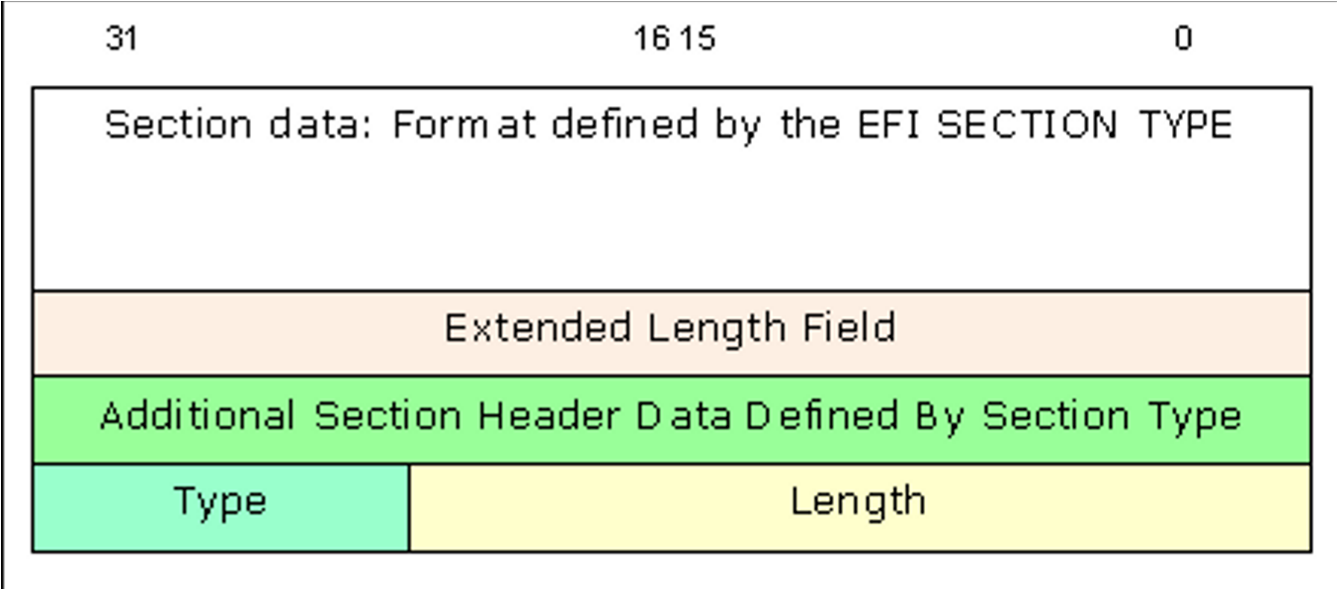
\includegraphics[width=0.7\linewidth]{design/general-efi-section-format-large}
	\caption{General EFI Section Format for large size Sections(greater then 16 MB)}\label{fig:design-general-efi-section-format-large}
\end{figure}


\begin{figure}[h]
	\centering
	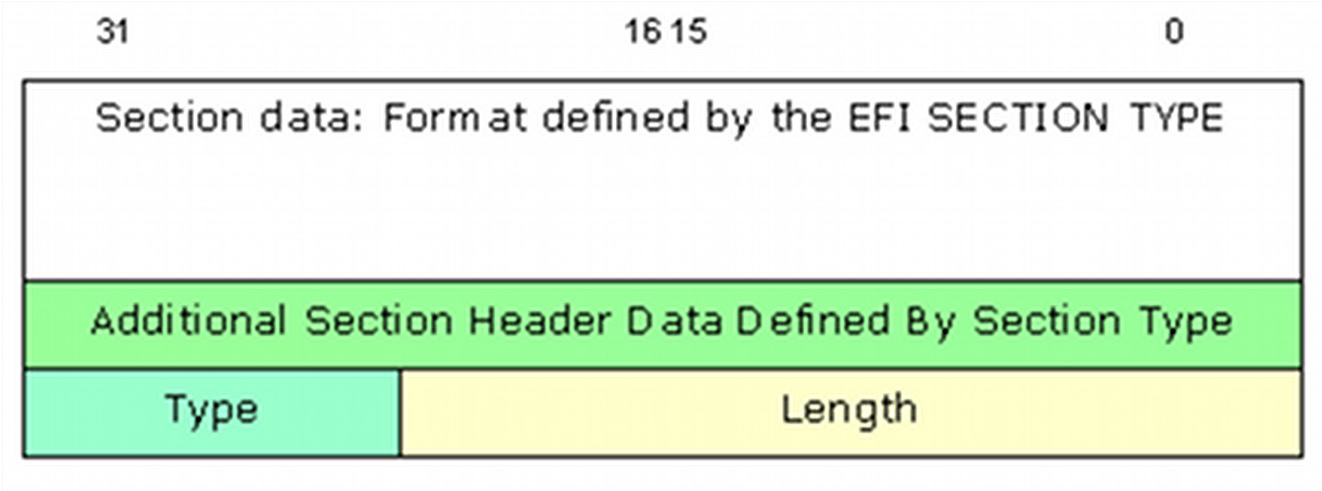
\includegraphics[width=0.7\linewidth]{design/general-efi-section-format}
	\caption{General EFI Section Format (less then 16 MB)}\label{fig:design-general-efi-section-format}
\end{figure}



\subsection{Cross Compatibility of CPUs}
Whenever customer try to change the default Intel motherboard CPU with different Intel silicon chip which won’t works. The specific CPU Chip initialization varies for each generation. So, the board designs should be designed is such a way that specific generation CPU should support., if we change the CPU with a different Intel Board it will not even boot, because the BIOS doesn't support for other Silicon Initialization for other CPUs.

So, we are integrating the runtime detection of the silicon during the Pre-Extensible Firmware Initialization (\gls{pei}) phase. So, within single Integrated Firmware Image (\gls{ifwi}) should support the Multi Generation CPUs which is never tried before.

Each silicon has a fixed register from which the CPU generation can be identified., so the BIOS should read that register and program in such a way the is CPU1 is in Platform it should support the CPU1 Features like PCIe, Graphics \& DMI., if the CPU1 is replaced with CPU2 then it should support the CPU2 speed. That should be taken care by the BIOS.

\begin{figure}[h]
	\centering
	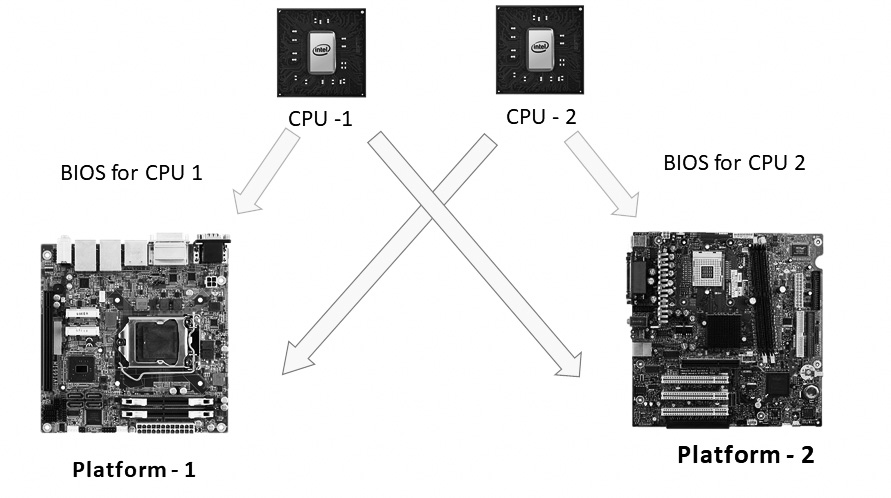
\includegraphics[width=0.7\linewidth]{design/cross-compatibility-design}
	\caption{Cross Compatibility Design}\label{fig:design-cross-compatibility-design}
\end{figure}

Figure \ref{fig:design-cross-compatibility-design} shows the general view of the Cross Compatibility of CPUs.

BIOS is the part of Integrated Firmware Image which resides at the End of the Binary table. The CPU swap can only occur in Specially designed Intel Designed Board only. Mainly because for each and every feature it required some hardware(H/W) requirements. If that H/W requirement not present. Then It will boot but doesn't support the Maximum speed.


\begin{figure}[h]
	\centering
	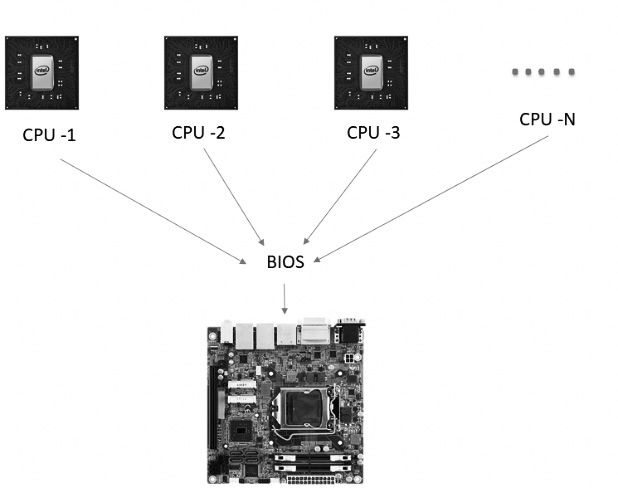
\includegraphics[width=0.7\linewidth]{design/bios-support-for-cross-compatibility}
	\caption{BIOS Support for Cross Compatibility}\label{fig:design-bios-support-for-cross-compatibility}
\end{figure}

Figure \ref{fig:design-bios-support-for-cross-compatibility} shows the BIOS role for identifying the CPUs during PEI phase.

As the number of Feature increases in the Silicon BIOS size also increases, usually the BIOS size varies from Platform to Platform and CPU to CPU., as we are integrating the Compatibility the BIOS size obviously increases. 

The structure of \gls{ifwi} is Shown in Figure \ref{fig:design-integrated-firmware-image}

\begin{figure}[h]
	\centering
	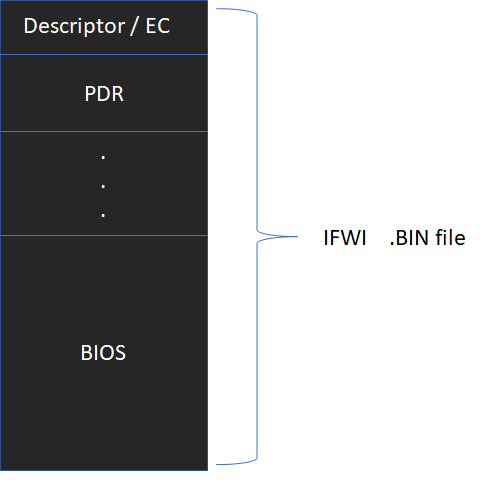
\includegraphics[width=0.7\linewidth]{design/integrated-firmware-image}
	\caption{Integrated Firmware Image}\label{fig:design-integrated-firmware-image}
\end{figure}




	\printglossary[type=main]
\end{document}